\chapter{Descripción del trabajo realizado}

Este capítulo consta de dos secciones principales. La primera presenta el
proceso seguido en función del marco metodológico: actividades realizadas,
retos encontrados, decisiones de diseño tomadas. La segunda sección presenta el
análisis de los resultados obtenidos por el proyecto, enfocado en comparar el
método de ML integrado en AxLS con otros métodos previamente existentes.

\section{Descripción del proceso de solución}

El proceso para llegar a la solución siguió la estructura planteada en el marco
metodológico, que la Figura \ref{fig:diagrama_metodológico} resume visualmente.

\subsection{Experimentación con AxLS}

El objetivo de esta actividad fue familiarizar al autor con la herramienta
AxLS, sus módulos existentes y formar una mejor idea de lo que tomaría el
proyecto. Se decidió intentar crear una prueba de concepto de lo que sería la
verdadera implementación de ML dentro de la herramienta, como ejercicio de
familiarización.
En el lapso de una semana se intentaría implementar un DT. Se
escogió utilizar un DT porque es una técnica fácil de utilizar correctamente,
cuya implementación ya existe en la biblioteca \emph{scikit-learn} y que se
entrena rápidamente.
La prueba de concepto fue exitosa, se logró realizar una síntesis aproximada de
uno de los circuitos de benchmark y se identificó cómo realizar los pasos
necesarios para la implementación de la técnica:

\begin{itemize}
  \item Sintetización del circuito original.
  \item Simulación del circuito original para obtener los datos de entrenamiento.
  \item Lectura de los datos de entrada y salida del circuito original para
    entrenar el árbol de decisiones.
  \item Entrenamiento del árbol de decisiones con implementación de
    \emph{scikit-learn}.
  \item Mapeo del árbol de decisiones a un circuito Verilog a través de
    expansión de Boole.
  \item Sintetización y simulación del circuito aproximado.
  \item Evaluación de técnicas de error.
\end{itemize}

Cabe notar que la técnica no estaba realmente integrada dentro de la
herramienta, ya que fue una implementación ad hoc. Además, presentaba varios
errores. Se decidió no dedicar más tiempo a intentar corregirlos, porque no
había certeza de que esa fuera la técnica final que se escogería para agregar
propiamente a AxLS.

\subsection{Escogencia de método ML}

Para escoger el método de ML, se siguieron los criterios planteados en el marco
metodológico, en la sección \ref{sec:seleccion_ml}. Después de una revisión
bibliográfica exhaustiva sobre técnicas de ML aplicadas a ALS, se realizó un
análisis explorando las diferentes técnicas utilizadas en el estado del arte.
Finalmente, se justificó cuál era la más apropiada para este proyecto.

\subsubsection{Escogencia de categoría}

Como se discute en la sección \ref{sec:trabajos_similares}, en la bibliografía
se identificaron 3 categorías principales de aplicación de métodos de ML en
ALS:

\begin{enumerate}
  \item Técnicas que entrenan modelos para asistir en otros métodos de ALS,
    acelerando la evaluación de errores al simular cambios en el circuito.
  \item Técnicas de ML aplicadas a la exploración del espacio de diseño de
    circuitos.
  \item Enfoques supervisados donde se entrena un modelo con entradas/salidas
    de un circuito, y luego se mapea a hardware.
\end{enumerate}

Para el método a implementar en la herramienta AxLS se escogió la categoría 3
debido a las siguientes consideraciones:

\begin{itemize}
  \item Se descartó completamente la categoría 2 por el criterio de
    viabilidad, ya que las exploraciones o entrenamientos realizados duran
    horas y son realizados en estaciones de trabajo considerablemente más
    potentes que lo que se tiene acceso para este proyecto.
  \item Luego se evaluaron más detenidamente los criterios de escogencia entre
    las categorías 1 y 3:
    \begin{itemize}
      \item Viabilidad: Por lo general los métodos de la categoría 3 tienen
        un entrenamiento menos extenso y más fáciles de realizar.
      \item Estado del arte: Hay considerablemente más trabajos de la
        categoría 3.
      \item Resultados: En ambas categorías hay resultados competitivos,
        ninguna es considerablemente más exitosa que la otra.
    \end{itemize}
\end{itemize}

\subsubsection{Escogencia de método}

Se evaluaron los métodos disponibles dentro de la categoría 3, y sus
consideraciones se discuten a continuación. En la sección
\ref{sec:trabajos_similares} se adentra más en los métodos de las otras
categorías.

\paragraph{Árbol de decisiones}

\begin{itemize}
  \item Es el método más estudiado en la literatura, 7 de las 10 referencias
    utilizadas lo estudian \cite{de_abreu_fast_2021, miyasaka_logic_2021,
    rai_logic_2021, zeng_sampling-based_2021, huang_circuit_2023,
    hu_optdtals_2024, prats_ramos_impact_2024}.
  \item Es muy viable debido a su fácil implementación, disponibilidad en
    bibliotecas de alto grado como \emph{scikit-learn} y bajo tiempo de
    entrenamiento. En efecto, ya se había realizado una implementación ad hoc
    como una prueba de concepto a inicios del proyecto.
  \item Tiene resultados competitivos. No siempre los mejores, pero por lo
    general la literatura lo menciona como una de las técnicas más efectivas
    o la base que están intentando superar con un método más avanzado.
\end{itemize}

Se consideró la posibilidad de implementar alguna de las versiones modificadas
que se han estudiado, como en \cite{hu_optdtals_2024} o
\cite{zeng_sampling-based_2021}, pero se decidió sería mejor implementar el
método más general para tener una base de comparación y dejar cualquier mejora
para un trabajo futuro.

\paragraph{Bosque aleatorio}

\begin{itemize}
  \item Fue explorada en 2 de las referencias estudiadas, las cuales son del
    2021 \cite{miyasaka_logic_2021}, \cite{rai_logic_2021}.
  \item Son fáciles de implementar, ya que están compuestos por DT.
  \item Sí ha obtenido mejores resultados que los DT en algunas de las tareas
    evaluadas dentro de las referencias, particularmente a la hora de
    generalizar circuitos lógicos y para algunos circuitos aritméticos en
    específico.
\end{itemize}

\paragraph{Programación genética cartesiana}

\begin{itemize}
  \item Esta técnica usa algoritmos evolutivos para generar circuitos,
    representando sus elementos como un \emph{genotipo} fácilmente mapeable
    al circuito final.
  \item Ha sido estudiada en 2 de las referencias utilizadas, las cuales son
    bastante modernas con la última siendo del 2024
    \cite{berndt_cgp-based_2022}, \cite{prats_ramos_impact_2024}.
  \item Esta técnica obtiene resultados muy exitosos en términos del
    intercambio entre área de circuito y error introducido.
  \item Se descartó por su alto costo computacional: incluso con un clúster
    mucho más potente que el equipo disponible, en
    \cite{berndt_cgp-based_2022} las ejecuciones tomaron hasta un día
    completo.
\end{itemize}

\paragraph{Perceptrón multicapa}

\begin{itemize}
  \item Esta técnica es explorada en 4 de las referencias utilizadas, con 3
    de ellas siendo del 2021 y la última del 2024
    \cite{boroumand_learning_2021}, \cite{miyasaka_logic_2021},
    \cite{rai_logic_2021}, \cite{prats_ramos_impact_2024}
  \item Su viabilidad es limitada por la dificultad de traducirlas a
    circuitos. Suelen requerir módulos complejos como sumadores y
    multiplicadores, lo que aumenta mucho el tamaño. Reducir esto implica
    técnicas como podar conexiones poco importantes o convertir cada nodo del
    MLP en una LUT mediante cuantización.
  \item Tienen buenos resultados en sus estudios, particularmente con
    circuitos aritméticos de adición y multiplicación y aprendiendo la
    operación lógica de XOR, tareas en las que los otros métodos suelen
    fallar.
\end{itemize}

\paragraph{Método escogido}

Tomando en cuenta las consideraciones dadas para cada método se decidió
implementar DT, principalmente por su alta viabilidad y relevancia dentro de la
literatura.

Se considera que además es una buena base para trabajo futuro en el que se implemente alguna variación de la técnica como RF, o las presentadas en \cite{hu_optdtals_2024}, \cite{zeng_sampling-based_2021} o \cite{huang_circuit_2023}.

\section{Implementación de técnica de ML}

Debido a la implementación previa de la técnica de DT como prueba de concepto,
la implementación real fue más fácil. Aun así, fue necesario integrarla
correctamente en AxLS, corregir errores y generalizarla para que funcionara con
cualquier circuito, no solo uno específico.

Se creó una clase llamada \texttt{DecisionTreeCircuit} que abstrae sobre la
implementación de DT de \emph{scikit-learn} para dar las utilidades necesarias
para realizar ALS. Esta solo expone los siguientes métodos:

\begin{itemize}
  \item \texttt{train(X, y)}: Acepta vectores con los datos obtenidos de la
    simulación del circuito original que utiliza para entrenar el árbol de
    decisiones interno.
  \item \texttt{to\_verilog\_file(topmodule, filename)}: Después de entrenar el
    árbol de decisiones, este método mapea el árbol entrenado a un circuito de
    Verilog y lo escribe en un archivo de texto especificado por el usuario. El
    parámetro de \texttt{topmodule} permite al usuario controlar el nombre del
    módulo de Verilog para el circuito.
\end{itemize}

Para que el árbol se adapte al circuito que se está aproximando y el módulo de
Verilog se genere correctamente, se deben suplir listas con las entradas y
salidas del circuito.
También se agregó el parámetro \texttt{one\_tree\_per\_output}, que permite
elegir entre un solo árbol multi-salida o uno por cada salida del circuito.
Esto se incluyó tras notar en la prueba de concepto que ambas opciones eran
posibles y afectaban el resultado.

La clase, sus propiedades y métodos se muestran en formato UML en la Figura
\ref{fig:UML}.

\begin{figure}[htb]
  \centering
  % El inkscapelatex=false evita que LaTeX trate de renderizar el texto,
  % necesario porque estaba tirando error por los underscores '_' en el svg.
  \includesvg[inkscapelatex=false, width=0.3\linewidth]{./imágenes/DecisionTreeCircuit_UML.svg}
  \caption{Representación de UML de \texttt{DecisionTreeCircuit}.}
  \label{fig:UML}
\end{figure}

El flujo completo de utilizar esta clase con las utilidades de AxLS conlleva los siguientes pasos, los cuales se representan visualmente en la Figura \ref{fig:flow}.

\begin{enumerate}
  \item Sintetizar circuito original con la clase \texttt{Circuit} ya existente dentro de AxLS.
  \item Simular el circuito original con un set de datos de entrada, generando las salidas correspondientes.
  \item Leer los archivos del set de datos de entrada y sus salidas correspondientes y entrenar el árbol de decisiones con estos.
  \item Mapear el árbol de decisiones a un circuito aproximado de Verilog.
  \item Sintetizar el circuito aproximado de Verilog con la clase \texttt{Circuit}. Con este objeto se pueden realizar simulaciones para obtener las métricas de área y error del circuito aproximado.
\end{enumerate}

\begin{figure}[htb]
  \centering
  % El inkscapelatex=false evita que LaTeX trate de renderizar el texto,
  % necesario porque estaba tirando error por los underscores '_' en el svg.
  \includesvg[width=0.6\linewidth]{./imágenes/decision_tree_method.svg}
  \caption{Representación visual de cómo utilizar \texttt{DecisionTreeCircuit} dentro de AxLS.}
  \label{fig:flow}
\end{figure}

Para validar la implementación se hicieron pruebas con un circuito sumador de 9
bits de entrada (dos entradas de 4 bits y 1 bit de acarreo). Las pruebas
examinaron los productos intermedios generados y el rendimiento del circuito
final para verificar su correcta implementación. Varias de las pruebas se
hicieron utilizando un DT sin profundidad máxima, que para este pequeño
circuito es capaz de memorizar todos los pares de entradas y salidas, generando
resultados exactos.

\begin{itemize}
  \item Se verificó que las entradas y salidas del circuito de Verilog generado
    calzaban correctamente a través de inspección manual y revisando que las
    salidas al simular el circuito coinciden con las salidas al manipular el DT
    en software directamente.
  \item Utilizando un DT sin profundidad máxima, se validó en software que
    las salidas correspondían con lo esperado dependiendo de las entradas. Por
    ejemplo si las entradas son ${3, 4, 1}$, la salida sería $8$ en binario.
  \item Utilizando un DT sin profundidad máxima, el circuito aproximado debería
    tener error de $0\%$ y se esperaría que tenga un área mayor al circuito
    original, ya que memorizar los pares de entradas y salidas es menos
    eficiente que programar la estructura de un sumador.
  \item Al reducir la profundidad máxima del DT, el área del circuito generado
    debía disminuir y el error aumentar.
\end{itemize}

\subsection{Recolección de resultados.}

Para la recolección de resultados, como se describió en la sección
\ref{sec:metodologia_resultados}, se definieron los resultados deseados y los
experimentos necesarios, se creó una API para proveer un uso más abstraído de
la herramienta AxLS, se creó una CLI que exponía la API para terminal y se
escribió software externo a la herramienta para la generación programática de
los resultados.

\subsubsection{Definición de experimentos}

El primer paso que se tomó como parte de la etapa de recolección de resultados
fue definir los resultados que se deseaban generar. Este paso era esencial para
definir las capacidades que debía exponer la API y los scripts externos que la
utilizarían.

En concordancia con el tercer objetivo específico, se buscó recolectar datos de
ejecución de la técnica de DT y de otros métodos dentro de la herramienta. Las
métricas medidas serían todas para las que la herramienta AxLS tiene soporte:

\begin{itemize}
  \item Área del circuito.
  \item Métricas de error del circuito:
    \begin{itemize}
      \item ER.
      \item MHD.
      \item WHD.
      \item MAE.
      \item MSE.
    \end{itemize}
\end{itemize}

También se decidió medir el tiempo de ejecución de cada método. La herramienta
AxLS no proveía soporte para esto directamente, ya que Python ofrece muchas
utilidades para medición de tiempo. Pero para la facilidad de los usuarios esta
métrica se agregó a la API de ejecución simplificada.

Los resultados recolectados siempre incluirían estas métricas. Se busca obtener
los mejores resultados posibles para cada uno de los métodos para realizar
una comparación justa. Se compararon los siguientes métodos, considerando las
variaciones a probar para sistemática intentar obtener los mejores resultados
para cada uno:

\begin{itemize}
  \item Métodos de poda: Esto incluye el resto de métodos previamente
    disponibles en AxLS. Para estos métodos se selecciona un umbral de error y
    se poda el circuito hasta alcanzar el umbral. Se probarían con y sin
    resíntesis, aunque según \cite{morales-monge_improving_2024}, la resíntesis
    casi siempre debería de ser beneficiosa.
  \item DT: Se decidió variar la máxima profundidad del árbol, si utilizar un
    solo árbol multi-salida o múltiples árboles con uno por salida y si aplicar
    resíntesis o no.
\end{itemize}

La intención era probar todos los métodos de poda disponibles dentro de la
herramienta AxLS, pero al experimentar se notó que \texttt{ccarving} y
\texttt{significance} requerirían mucha configuración para obtener resultados
óptimos. Esto es debido a que estos métodos se basan en una métrica de
``significancia'' para escoger cuáles nodos de un circuito podar, la cual se
asigna a los nodos del circuito basado en una entrada de las significancias de
cada salida. Se decidió que seleccionar manualmente la significancia de las
salidas de manera óptima para todos los circuitos que se probarían se sale del
alcance de este proyecto. El método \texttt{ccarving} también podría utilizar
métricas diferentes, pero también se decidió que evaluar diferentes métricas
para este método se sale del alcance del proyecto.

Como los métodos de poda tienen un umbral de error controlable, pero el método
de DT no, es que se prueban múltiples profundidades máximas para este método.
Al permitir mayor profundidad de árbol, se espera que el árbol haga un mejor
trabajo de aprender la función, reduciendo su error a pesar de que el circuito
final requiera más área.

\subsubsection{Creación de API simplificada y CLI}

Para la creación de la API simplificada para la ejecución de AxLS, en base con
los resultados que se desean generar y en general permitir una ejecución
configurable de los métodos de AxLS, se definieron los siguientes
requerimientos:

\begin{itemize}
  \item Poder ejecutar cualquiera de los métodos dentro de AxLS:
    \begin{itemize}
      \item \texttt{ccarving}: Tallado de circuitos, como se presenta en
        \cite{scarabottolo_circuit_2018}.
      \item \texttt{significance}: Poda a nivel de compuertas basado en
        significancia, como se presenta en \cite{schlachter_design_2017}.
      \item \texttt{inconst}: Poda nodos del circuito bajo la suposición de que
        algunas entradas son constantes. Al ejecutarlo a través de la API se
        inicia asumiendo que los bits de entrada menos significativos son
        constantes y al podar todos los nodos sugeridos se asume que el
        siguiente bit es constante y se continúa hasta alcanzar alguna
        condición de parada.
      \item \texttt{outconst}: Igual que \texttt{inconst}, pero asumiendo que
        algunas de las salidas son constantes.
      \item \texttt{probprun}: Basado en información de temporización adquirida
        a través de la simulación de circuitos, recomienda podar nodos en función
        del tiempo que permanecieron en un valor específico, 0 o 1, lo que
        indica los nodos que asumieron un valor particular la mayor parte del
        tiempo.
      \item \texttt{decision\_tree}: El método de DT.
    \end{itemize}
  \item Aceptar todos los parámetros de configuración necesarios de cada
    método.
    \begin{itemize}
      \item Parámetros que todos los métodos aceptan: Si utilizar resíntesis, si
        separar el set de datos en un set de prueba y otro de validación.
      \item En común para todos los métodos de poda: Umbral de error, cuántos
        nodos podar en cada iteración.
      \item \texttt{ccarving} y \texttt{significance}: Una lista de las
        significancias de cada bit de salida.
      \item \texttt{decision\_tree}: Profundidad máxima del árbol, si utilizar un
        árbol multi-salida o múltiples árboles con uno para cada salida.
    \end{itemize}
  \item Medir el tiempo de las ejecuciones y ofrecerlo como una de las métricas
    medibles al ejecutar un método.
  \item Controlar mostrar el progreso de las simulaciones de los circuitos.
  \item Capacidad de generar un CSV con los resultados de la ejecución, o
    agregar los datos a un CSV existente.
\end{itemize}

Se decidió separar el set de datos en uno de prueba y otro de validación
porque, en circuitos grandes, no es posible generar todas las combinaciones
posibles de entradas. Esto se debe a que la cantidad de entradas crece de forma
exponencial con la fórmula $2^n$ donde $n$ es la cantidad de bits de entrada.
Por eso, se permite dividir el set de datos para usar una parte en validar si
el método funciona bien con entradas que no se vieron durante la ejecución.

Esta técnica es común en el dominio de ML, ya que ayuda a saber si un modelo
generaliza bien o si está muy ajustado a los datos con los que fue entrenado.
En este caso se usó principalmente para evaluar la capacidad de generalización del método de DT, pero también sirve con los métodos de poda.
Ahí ayuda a ver si el umbral de error alcanzado se debe solo al set de prueba o
si en realidad representa bien lo que haría el circuito con cualquier entrada.
En el caso de \texttt{probprun}, que trabaja con datos simulados, el set de
validación permite comprobar si el circuito aproximado solo funciona bien con
esos datos o si generaliza bien a cualquier entrada.

El requerimiento de poder controlar si se muestra el progreso de las
simulaciones se agregó porque AxLS solía siempre mostrar el progreso de las
simulaciones a través de la terminal, pero con experimentación se notó que si
no mostraba el progreso entonces la simulación se ejecuta más velozmente. Igual
se mantuvo la opción de mostrar el progreso si se desea para motivos de depurar
errores o simplemente querer saber el progreso de una ejecución.

La opción para agregar los resultados obtenidos a un CSV se agregó por motivos
de generación de resultados. Se decidió utilizar el formato CSV porque es
ampliamente utilizado, legible por humanos y por máquinas, fácil de entender,
fácil de generar y tiene soporte de muchas herramientas.

Todas estas opciones fueron fáciles de exponer a través de una CLI. A la API
simplificada no se le agregaron opciones para generación de sets de datos porque
AxLS ya previamente proveía una API muy simple para esto, la cual
adicionalmente se expuso a través de la CLI para fácil generación de sets de
datos para simulación.

Para validar la implementación de la API se probó ejecutar todos los métodos de
manera manual con programas de Python que utilizan AxLS como biblioteca y a
través de la CLI. Al utilizar el mismo set de datos al aproximar un circuito
con el programa y con la CLI, todos generaron circuitos idénticos.

\subsubsection{Generación de resultados}

Al finalizar la API para ejecutar los métodos de AxLS, se empezó a trabajar en
la generación de los resultados deseados.

El primer paso era generar los sets de datos que se utilizarían para cada
circuito. Para circuitos pequeños, aquellos con 16 bits de entrada o menos, se
pueden generar todas las entradas posibles que pueden tener.
Por lo tanto, para los circuitos pequeños se generaron sets de datos
exhaustivos, que contienen todas las entradas posibles del circuito.
Para lograr esto se tuvo que agregar funcionalidad adicional a AxLS para poder
generar sets de datos sin repetición.

Para circuitos grandes se vuelve imposible utilizar sets de datos exhaustivos o
representativos. Por ejemplo, en un circuito de 32 bits de entrada, hay \num{4.3e9}
posibles entradas al circuito. Aunque se utilice un set de datos de 1 millón de
entradas, eso solo representaría un $2.3\%$ de las entradas posibles del
circuito. Para circuitos mayores es mucho peor, debido al crecimiento
exponencial de la cantidad de posibles entradas, para un circuito de 64 bits o
128 bits de entrada se vuelve completamente inviable generar un set de datos
representativo. Generar un $1\%$ de sus posibles entradas requeriría más memoria
de la que tiene cualquier disco duro moderno.

Otro motivo que complica usar grandes sets de datos es que entre más grande sea
el circuito, más procesamiento requiere simularlo. Un circuito siempre se tiene
que simular al final de una ejecución para medir sus métricas de error. Además,
el método \texttt{probprun} requiere una simulación previa para recolectar
datos de temporización. Y posiblemente lo peor es que todos los métodos de poda
requieren múltiples simulaciones debido al proceso que siguen:

\begin{enumerate}
  \item Podar uno o múltiples nodos.
  \item Simular el circuito podado para evaluar el error introducido.
  \item Si el error introducido es menor al umbral definido, volver al paso 1.
  \item Si el error es mayor al umbral definido, se reincorporan los últimos
    nodos podados hasta que el error vuelva a estar por debajo del umbral.
\end{enumerate}

Este procedimiento también se muestra visualmente en la Figura
\ref{fig:flow_poda}.

\begin{figure}[htb]
  \begin{center}
    \includesvg[width=0.5\textwidth]{./imágenes/prune_flowchart.svg}
  \end{center}
  \caption{Diagrama de flujo del proceso seguido con los métodos de poda.}
  \label{fig:flow_poda}
\end{figure}

Tomando en cuenta estas limitaciones, se tuvo que definir de qué tamaño hacer
los sets de datos para evitar problemas durante la ejecución. Como la
simulación de los circuitos es una de las etapas que más tiempo consume,
especialmente en los métodos de poda, se decidió que el tamaño del set de datos
dependiera de cuánto tardaba la simulación.

Con eso en mente, se hicieron simulaciones de \num{1000} elementos para medir
cuánto tardaba, en promedio, cada circuito en procesar un solo elemento. Con
ese dato se estimó el tamaño adecuado de los sets de datos. Los resultados de
esta prueba se muestran en el apéndice, en la Tabla \ref{tab:timing_info}. Se
escogió arbitrariamente un tiempo de simulación de $\SI{2}{\second}$ como un
límite corto que permitiera ejecutar los métodos de poda en un tiempo razonable.
Para el método \texttt{decision\_tree} se utilizó un set de datos más grande,
ya que no tiene que realizar tantas simulaciones y un método ML se beneficia
mucho más de tener mayor cantidad de datos. Se optó por un set de datos que
correspondiera con una simulación de $\SI{20}{\second}$ como un tamaño
considerablemente más grande, pero que no fuese a causar tiempos de ejecución
demasiado largos.

Basado en esa prueba, se decidió excluir algunos circuitos del resto del
proceso de recolección de resultados. La mayoría se descartaron por ser
demasiado lentos en simulación; algunos incluso se cancelaron sin terminar.
Otros sí completaron la prueba, pero fueron eliminados porque el set de datos
que se podía generar para $\SI{2}{\second}$ de simulación era demasiado pequeño
y no podría representar bien el error introducido. También se excluyeron algunos
porque no estaban funcionando bien. Finalmente, unos pocos se descartaron
aunque sí se podían simular en $\SI{2}{\second}$, ya que los métodos de poda
nunca lograron completarse y fue necesario cancelarlos después de horas sin
alcanzar el umbral de error. La Tabla \ref{tab:exclusiones} detalla las razones
por las que se excluyó cada circuito.

\begin{table}[htb]
  \centering
  \caption{Circuitos excluidos de la recolección de resultados y sus motivos.}
  \label{tab:exclusiones}
  \begin{tabular}{M{0.2\linewidth}M{0.5\linewidth}}
    \toprule
    Circuito & Motivo de exclusión \\
    \midrule
    hyp\_128b &  \multirow{4}{\linewidth}{Demasiado lentos en simular, no
    terminaron la prueba de \num{1000} datos de entrada.} \\
    sqrt\_128b & \\
    mul\_64b & \\
    log2\_32b & \\
    \midrule

    div\_64b &        \multirow{7}{\linewidth}{Lentos en simular, el set de
    datos generado para una simulación de $\SI{2}{\second}$ sería de menos de
    mil datos.} \\
    square\_64b &            \\
    fwrdk2j &                \\
    Mul\_32b &              \\
    sin\_24b &              \\
    voter &                  \\
    RForest &                \\
    \midrule

    max\_128b &       \multirow{2}{\linewidth}{Por su complejidad, los métodos
    de poda duraron demasiado y se cancelaron. }       \\
    adder\_128b &            \\
    \midrule
    invk2j & \multirow{2}{\linewidth}{Tienen errores que no permiten sintetizar
    o simular correctamente.} \\
    fir &  \\
    \bottomrule
  \end{tabular}

\end{table}

Otro cuello de botella identificado es la creación de archivos en formato SAIF
\cite{amd_vivado_2024}. Estos archivos contienen la información de
temporización que usa el método \texttt{probprun}. Para generarlos, primero se
debe simular el circuito deseado. Durante esta simulación, se escribe la
información de ejecución en un archivo VCD. Este archivo guarda los cambios de
valor de cada nodo del circuito \cite{noauthor_ieee_nodate}, así que su tamaño
crece dependiendo del tamaño del circuito y de cuántos datos de entrada se usen
en la simulación.

Una vez generado el archivo VCD, este se utiliza como base para crear el
archivo SAIF.

Para convertir un archivo VCD a SAIF, AxLS incluye un script en Python llamado
\texttt{vcd2saif.py}. Se verificó mediante una prueba sencilla que, entre más
grande sea el set de datos, más tiempo toma ejecutar esta conversión. Los
resultados de esa prueba se muestran en la Tabla \ref{tab:vcd2saif}.

\begin{table}[htb]
  \centering
  \caption{Pruebas de tiempo de ejecución de \texttt{vcd2saif.py} en el archivo VCD generado con el circuito BK\_16b.}
  \label{tab:vcd2saif}

  \begin{tabular}{M{0.2\linewidth}M{0.2\linewidth}}
    \toprule
    Tamaño de set de datos simulado & Tiempo de ejecución (\si{\milli\second}) \\
    \midrule
    \num{1000} & \num{7.60} \\
    \num{4000} & \num{29.54} \\
    \bottomrule
  \end{tabular}
\end{table}

Tomando en cuenta que la simulación de \num{4000} datos para este circuito dura
menos de $\SI{200}{\milli\second}$, pero la generación del archivo SAIF toma
casi medio minuto, se decidió que valía la pena intentar acelerar este proceso.
Al revisar la función en Python, se notó que no hace nada muy complejo, pero sí
recorre línea por línea todo el archivo VCD. Estos archivos crecen muy rápido.
Por ejemplo, para el circuito BK\_16b, con una simulación de \num{4000}
combinaciones de entrada, el archivo VCD llega a tener \num{724000} líneas.

Como Python es conocido por ser lento, se decidió reescribir la utilidad
\texttt{vcd2saif} en un lenguaje más rápido. Los principales candidatos fueron
lenguajes compilados como C, Go y Rust. Se eligió Rust porque el autor ya tenía
experiencia con él, ofrece buen rendimiento y tiene muchas herramientas útiles
para escribir una CLI de forma rápida \cite{bugden2022rust}.

Una vez terminada la nueva versión en Rust, llamada \texttt{vcd2saif\_rs}, se
repitió el experimento con el circuito BK\_16b y \num{4000} datos de entrada.
La utilidad en Rust tardó solo $\SI{1.43}{\second}$ en una tarea que con la
versión en Python tomaba casi medio minuto. Gracias a esto, el tiempo de
generación del archivo SAIF se redujo a aproximadamente una vigésima parte del
original.

Se cronometraron las ejecuciones de \texttt{vcd2saif\_rs} para todos los
circuitos con archivo SAIF generado; los resultados se incluyen en el apéndice,
en la Tabla \ref{tab:vcd2saif_rs}.
Si se suman esas ejecuciones la generación de archivos SAIF duró hora y media.
Asumiendo que el script de Python dura 20 veces más, hubiera durado alrededor
de 31 horas. Con estos datos se evidencia que traducir el script a Rust fue
sumamente beneficioso para la realización del proyecto.

Finalmente, tras realizar los experimentos definidos previamente, se
recolectaron los datos necesarios para evaluar el desempeño de la técnica
implementada. A continuación, se presenta un análisis detallado de los
resultados obtenidos.

\section{Análisis de los resultados obtenidos}

En esta sección se analizan los resultados de los experimentos descritos
previamente. Primero se comparan variantes del método DT: con o sin resíntesis,
y usando un solo árbol multi-salida o uno por salida. Luego se contrasta DT
contra otros métodos de AxLS, evaluando métricas de área, error y tiempo.
También se discute en qué tipos de circuitos la técnica de DT destaca y en
cuáles no funciona.

\subsubsection{Variaciones en DT}

\paragraph{Resíntesis}

La primera variación que se evaluó fue si utilizar resíntesis en el circuito
aproximado generado por el método \texttt{decision\_tree} es beneficioso.

La Figura \ref{fig:resynth} muestra una comparación en métricas de error, área y
tiempo de ejecución.

\begin{figure}
  \centering
  \begin{subfigure}{0.95\textwidth}
    \centering
    \includesvg[inkscapelatex=false, width=\textwidth]{./imágenes/mred_resynthesis_comparison.svg}
    \caption{Comparación del error introducido.}
    \label{fig:resynth_mred}
  \end{subfigure}
  \begin{subfigure}{0.95\textwidth}
    \centering
    \includesvg[inkscapelatex=false, width=\textwidth]{./imágenes/area_resynthesis_comparison.svg}
    \caption{Comparación del área resultante.}
    \label{fig:resynth_area}
  \end{subfigure}
  \begin{subfigure}{0.95\textwidth}
    \centering
    \includesvg[inkscapelatex=false, width=\textwidth]{./imágenes/time_resynthesis_comparison.svg}
    \caption{Comparación del tiempo de ejecución.}
    \label{fig:resynth_time}
  \end{subfigure}
  \caption{Resultados de aplicación de resíntesis con método \texttt{decision\_tree}.}
  \label{fig:resynth}
\end{figure}

El patrón observado en el error
es que hay algunas variaciones mínimas, puede ser ligeramente mayor
o menor con resíntesis. Como las variaciones son tan pequeñas y no son
constantes se atribuyen a un elemento aleatorio en el entrenamiento del DT.
Esto es el comportamiento esperado, ya que la resíntesis no debería de afectar
las salidas que produce un circuito.

En un entorno práctico no interesarían los casos donde el área del circuito
resultante sobrepase el 100\% del área del circuito original, pero igualmente
se incluyeron esos casos en la gráfica para mejor estudiar el efecto de
resintetizar un circuito. Se observa el mismo patrón que con el error, los
valores son muy parecidos en la mayoría de casos con variaciones pequeñas que
no son consistentes entre los casos de con y sin resíntesis, por lo que se
atribuyen a la aleatoriedad del DT.

En el caso del área sí se esperaba obtener más
beneficios de la resíntesis, ya que se esperaba que el DT generara estructuras
no tan eficientes y el proceso de resintetizar el circuito pudiera reacomodar
los nodos de mejor manera y evitando algunas redundancias. Sin embargo, parece
que este no fue el caso, implicando que el resultado del DT no se puede reducir
más.

Finalmente, para la comparación de tiempo se tiene un resultado similar, no hay
variaciones muy significativas en la mayoría de casos, con la excepción de
árboles muy profundos en circuitos muy complejos. Conforme el árbol crece en
complejidad, es de esperarse que el tiempo de ejecución aumente
considerablemente. Esto se debe a que el tiempo de síntesis crece respecto a la
complejidad del circuito. Como se ha mencionado previamente, el DT crece en
complejidad exponencialmente con su profundidad. Además, un circuito complejo
resulta en tiempos de síntesis muy largos, lo que opaca, en términos de tiempo,
el resto de los procesos de la ejecución de ALS.

Sin embargo, los casos donde la resíntesis tiene un efecto considerable en el
tiempo de ejecución son los casos donde el área del circuito resultante
sobrepasa el 100\% del área del circuito original, por lo que no son casos de
interés práctico.

En general, se observó que resintetizar el circuito resultante generado por el
método \texttt{decision\_tree} no tiene efectos significativos, ni positivos ni
negativos.

\paragraph{Múltiples árboles}

La otra variación que se estudió para el método \texttt{decision\_tree} fue si
entrenar un solo árbol multi-salida para representar el circuito completo, o si
entrenar un árbol diferente que solo aprendiera una de las salidas del
circuito.

La Figura \ref{fig:one_tree_per_output} muestra una comparación en métricas de
error, área y tiempo de ejecución.

\begin{figure}
  \centering
  \begin{subfigure}{0.95\textwidth}
    \centering
    \includesvg[inkscapelatex=false, width=\textwidth]{./imágenes/mred_one_tree_per_output_comparison.svg}
    \caption{Comparación del error introducido.}
    \label{fig:one_tree_per_output_mred}
  \end{subfigure}
  \begin{subfigure}{0.95\textwidth}
    \centering
    \includesvg[inkscapelatex=false, width=\textwidth]{./imágenes/area_one_tree_per_output_comparison.svg}
    \caption{Comparación del área resultante.}
    \label{fig:one_tree_per_output_area}
  \end{subfigure}
  \begin{subfigure}{0.95\textwidth}
    \centering
    \includesvg[inkscapelatex=false, width=\textwidth]{./imágenes/time_one_tree_per_output_comparison.svg}
    \caption{Comparación del tiempo de ejecución.}
    \label{fig:one_tree_per_output_time}
  \end{subfigure}
  \caption{Resultados de utilizar un árbol por salida comparado con un solo árbol multi-salida usando el método \texttt{decision\_tree}.}
  \label{fig:one_tree_per_output}
\end{figure}

En la gráfica de error se observa que por lo general produce mejores resultados
utilizar un solo árbol multi-salida. Esto es lo que se esperaba, ya que al
utilizar un solo árbol este explota mejor las correlaciones entre las salidas
del circuito dada una entrada. Si no hubiese correlaciones entre las salidas
entonces no habría beneficio, pero los bits de salida de un circuito se
esperaría que estén altamente correlacionados entre sí.
Cabe notar el caso del circuito \texttt{WT\_8b}, que es el único que ve una
clara mejora al usar árboles separados para cada salida. Este circuito es un
multiplicador, lo cual implica que las salidas de la operación de multiplicación
no presenta correlación entre sus salidas.

Por otro lado, el área del circuito siempre se ve afectada negativamente, i.e.
al utilizar un árbol diferente por salida, el área siempre resulta mayor. Esto
incluso con el circuito \texttt{WT\_8b}, significando que su disminución en
error fue un compromiso al costo de mayor área.

% TODO: Frente pareto para WT_8b donde los nodos de un árbol y los de muchos
% árboles tienen colores diferentes?

Utilizar un árbol por salida resultó en tiempos de ejecución considerablemente
más lentos. Esto se atribuye a que se deben entrenar varios DT en vez de solo
uno y probablemente producen un circuito más complejo que el que produce un
solo árbol resultando en tiempos de síntesis mayores.

\subsubsection{DT contra métodos de poda}

A continuación se compara el método \texttt{decision\_tree} agregado a la
herramienta contra métodos de poda ya previamente disponibles:
\texttt{inconst}, \texttt{outconst}, \texttt{probprun}.

También se discute en qué circuitos \texttt{decision\_tree} funciona mejor y en
cuáles no funciona.

Una característica clave de los métodos de poda en comparación al método de DT
es que ellos permiten controlar el error introducido al circuito con un umbral
de error definido por el usuario y realizan cambios incrementales en el
circuito hasta alcanzarlo. A diferencia del método DT que reemplaza el circuito
entero y el área y error del circuito aproximado producido no se puede
controlar más allá de variar los parámetros del DT hasta obtener los resultados
más cercanos a los deseados.

Por esta limitación del DT, para poder realizar comparaciones lo más
equivalentes posible, los métodos de poda se ejecutaron con múltiples umbrales
de error diferentes: \num{1}\%, \num{5}\%, \num{10}\%, \num{25}\% y \num{50}\%.
Así se pueden escoger las ejecuciones de métodos de poda que tengan un umbral de
error similar a los resultados obtenidos por DT.

La Tabla \ref{tab:1_porciento} muestra los mejores resultados de cada método
evaluado con un umbral de error del 1\%. Para esta y próximas tablas, el mejor
resultado sería aquel con la menor área entre los resultados con error menor al
umbral. En general también solo se incluirán los circuitos en los que el método
\texttt{decision\_tree} logró producir un resultado con error por debajo del
umbral y con área menor al 100\% del área original. En el caso de la Tabla
\ref{tab:1_porciento} solo se incluyen los circuitos RCA\_4b e int2float porque
en ningún otro el método \texttt{decision\_tree} pudo producir un circuito
aproximado con error tan bajo. Esta incapacidad del método de DT de producir
resultados con un error controlado limita los circuitos en los que puede ser
efectivo. Sin embargo, vemos que los circuitos con los que el método
\texttt{decision\_tree} sí obtiene un error por debajo de 1\% tienen resultados
muy positivos en términos de la reducción del área.

Para el circuito RCA\_4b todos los métodos encontraron una variación del
circuito que tenía 0\% de error, pero tenía área reducida, con el método de DT
sobresaliendo en la reducción del área. Cabe tomar en cuenta que este circuito
tiene solo 9 bits de entrada, por lo que se utilizó el set de datos exhaustivo
de las posibles entradas del circuito para medir el error, lo que significa que
realmente el circuito original tenía redundancias.

Con el circuito int2float la diferencia es más marcada, \texttt{outconst} y
\texttt{probprun} reducen el área en \num{1.46}\%, \texttt{inconst} en
\num{19.57}\% y \texttt{decision\_tree} en \num{33.95}\%. Esto indica que
cuando el método basado en DT sí funciona, obtiene muy buenos resultados en
comparación a los métodos de poda.
Algo sorprendente en este caso es que los mejores resultados provienen de
ejecuciones con un árbol diferente por salida y de mucha profundidad.

Estos dos circuitos son de naturaleza diferente, int2float es un circuito
lógico y RCA\_4b es un sumador aritmético. Lo que tienen en común es ser de los
circuitos más pequeños entre los benchmarks disponibles para AxLS. Solo hay
otro circuito de menos de 16 bits de entradas disponible para pruebas: un
decodificador de 8 bits con 256 bits de salida. Con el decodificador el DT solo
pudo generar un circuito con más área que el original con 0\% de error, o
generar un circuito que solo genera valores de 0 en la salida, por lo que no se incluyó
en los resultados.

Esto indica que el DT es especialmente efectivo para circuitos pequeños y
posiblemente con el decodificador no pudo ser efectivo debido a su gran
cantidad de bits de salida. También, se observa que si se tiene la necesidad de
mantener un bajo error para estos circuitos pequeños, es posible que
permitirle al método de DT formar estructuras más complejas (con mayor
profundidad y usando árboles separados por cada salida) le puede permitir
encontrar caminos más eficientes para aprender el set de datos limitado.

\begin{table}[htb]
  \centering
  \caption{Comparación de métodos de AxLS para umbral de 1\% de error.}

% LTeX: enabled=false

  \label{tab:1_porciento}

  %\resizebox{\textwidth}{!}{

  \begin{tabular}{c S c S<{\%}S<{\%}S<{\%}S<{\%}}
    \toprule
    \multirow{2}{*}[-5pt]{Circuito} &
    \multicolumn{3}{c}{\texttt{decision\_tree}} &
    \multicolumn{1}{c}{\texttt{inconst}} &
    \multicolumn{1}{c}{\texttt{outconst}} &
    \multicolumn{1}{c}{\texttt{probprun}} \\
    \cmidrule(lr){2-4}
    \cmidrule(lr){5-5}
    \cmidrule(lr){6-6}
    \cmidrule(lr){7-7}
    &
    \multicolumn{1}{M{2cm}}{Profundidad máxima} &
    \multicolumn{1}{M{2cm}}{Un árbol por salida} &
    \multicolumn{1}{c}{Área} &
    \multicolumn{1}{c}{Área} &
    \multicolumn{1}{c}{Área} &
    \multicolumn{1}{c}{Área} \\
    \midrule

    RCA\_4b & 10 & Sí & 94.78 & 98.51 & 98.51 & 98.51 \\
    int2float & 8  & Sí & 66.05 & 80.43 & 98.54 & 98.54 \\

    \bottomrule
  \end{tabular}

  %}
\end{table}
% LTeX: enabled=true

De aquí saltamos al umbral de 25\%, ya que \texttt{decision\_tree} no logró
generar resultados para nuevos circuitos en los umbrales de 5\% y 10\%. Se
presentan los mejores resultados obtenidos en la Tabla \ref{tab:25_porciento}.

\begin{table}[htb]
  \centering
  \caption{Comparación de métodos de AxLS para umbral de 25\% de error.}

  % LTeX: enabled=false

  \label{tab:25_porciento}

  %\resizebox{\textwidth}{!}{

  \begin{tabular}{c S c S<{\%}S<{\%}S<{\%}S<{\%}}
    \toprule
    \multirow{2}{*}[-5pt]{Circuito} &
    \multicolumn{3}{c}{\texttt{decision\_tree}} &
    \multicolumn{1}{c}{\texttt{inconst}} &
    \multicolumn{1}{c}{\texttt{outconst}} &
    \multicolumn{1}{c}{\texttt{probprun}} \\
    \cmidrule(lr){2-4}
    \cmidrule(lr){5-5}
    \cmidrule(lr){6-6}
    \cmidrule(lr){7-7}
    &
    \multicolumn{1}{M{2cm}}{Profundidad máxima} &
    \multicolumn{1}{M{2cm}}{Un árbol por salida} &
    \multicolumn{1}{c}{Área} &
    \multicolumn{1}{c}{Área} &
    \multicolumn{1}{c}{Área} &
    \multicolumn{1}{c}{Área} \\
    \midrule

    int2float & 3 & No & 5.19 & 7.57 & 36.09 & 20.91 \\
    BK\_16b & 3 & No & 26.85 & 10.51 & 49.42 & 84.44 \\
    KS\_16b & 4 & No & 44.15 & 8.00 & 35.41 & 58.07 \\
    CSkipA\_16b & 3 & No & 29.57 & 10.51 & 49.22 & 87.94 \\
    LFA\_16b & 4 & No & 54.86 & 8.75 & 48.44 & 98.83 \\
    CLA\_16b & 3 & No & 29.60 & 8.27 & 43.93 & 73.53 \\
    BK\_32b & 3 & No & 23.22 & 4.28 & 42.06 & 80.88 \\
    KS\_32b & 4 & No & 43.01 & 3.44 & 35.91 & 52.48 \\

    \bottomrule
  \end{tabular}

  %}
\end{table}
% LTeX: enabled=true

Cabe notar que para este umbral, todos los mejores resultados dados por el
método \texttt{decision\_tree} son utilizando un solo árbol multi-salida. Esto
se alinea más con lo observado previamente respecto al uso de un árbol
multi-salida comparado a múltiples árboles.
Para este nuevo umbral el método de DT sigue generando el mejor resultado para
int2float, en el resto se mantiene competitivo respecto a \texttt{outconst} y
\texttt{probprun}, pero \texttt{inconst} es el ganador por mucho.

El circuito RCA\_4b no fue incluido porque la mejor respuesta de
\texttt{decision\_tree} para el umbral de 25\% continúa siendo la misma
presentada en la Tabla \ref{tab:1_porciento}.

Todos los circuitos incluidos con los que \texttt{decision\_tree} logró obtener
un error de menos del 25\%, aparte de int2float, son circuitos sumadores que
reciben dos entradas de 32 o 16 bits.
Los circuitos con los que no logró obtener resultados por debajo de este error
son:

\begin{itemize}
  \item WT\_8b: Un multiplicador de 2 entradas de 8 bits.
  \item sobel: Un circuito que aplica un filtro detector de bordes que recibe
    una entrada de 81 bits.
  \item DTree: Un DT entrenado que recibe 30 entradas de 10 bits cada una.
  \item barshift\_128b: Desplazador de barril de 7 bits a la izquierda para entradas de 128 bits.
\end{itemize}

% TODO: Podría probar DT con otros circuitos que los de poda no terminaron
% nunca. Ponerlo como un beneficio del método DT o poder analizar mejor cuáles
% circuitos sirven vs cuáles no.

La imposibilidad de generar un resultado para WT\_8b que pudiera incluirse en la
Tabla \ref{tab:25_porciento} sugiere que a un árbol de decisión (DT) le cuesta
especialmente aprender la operación de multiplicación, incluso cuando se trata
de un circuito relativamente pequeño. Esto indica que a un DT le resulta más
sencillo aprender sumas que multiplicaciones, ya que los circuitos sumadores
que sí aparecen en la tabla manejan entradas mucho más grandes que el WT\_8b.
Lo reportado en \cite{miyasaka_logic_2021} concuerda con esta observación,
donde se muestra que los RF, formados por múltiples DT, también fallan al
intentar aprender multiplicaciones. Esta dificultad se atribuye a que los bits
de salida en una multiplicación suelen depender de operaciones XOR, las cuales
presentan poca información mutua entre entradas y salidas, complicando su
aprendizaje para modelos como los DT, que se basan precisamente en la
información mutua para dividir los datos.

La exclusión de los circuitos sobel, barshift\_128b y DTree parece indicar que
el método falla en crear circuitos satisfactorios para circuitos muy grandes.
La exclusión del método DTree es especialmente sorprendente porque es una
estructura de DT y lo estamos aproximando con un DT.

Se podría analizar más el porqué no se logra crear una aproximación útil.
Algunos posibles motivos son que se requiere un DT bastante más complejo que
los que se probaron, debido a la gran cantidad de información de entrada.
También podría ser que faltó utilizar más datos de entrenamiento o que se usó
una estrategia diferente para sintetizar el DT original a un circuito, como
reutilizar módulos comparadores en vez de convertir el árbol en un SOP, que es
la estrategia utilizada por \texttt{decision\_tree}.

La exclusión de los circuitos sobel, barshift\_128b y DTree sugiere que el
método no logra generar aproximaciones satisfactorias para circuitos muy
grandes. La exclusión del circuito DTree resulta especialmente sorprendente, ya
que originalmente es una estructura de DT adaptada a circuito, y estamos
intentando aproximarla precisamente con un DT. Esto podría deberse a varios
factores: tal vez se requiere un DT más complejo que los evaluados,
debido a la alta cantidad de entradas; podría ser que se necesitaban más datos
de entrenamiento; o también podría ser que la síntesis del DT original se hizo
con una estrategia distinta, como reutilizar módulos comparadores en lugar de
convertir el árbol a una forma SOP, que es la estrategia empleada por
\texttt{decision\_tree}.

% TODO: Relacionado al TODO anterior, podría probar con circuitos grandes que no
% la dieron para los de poda para ver si se mantiene la hipótesis.
% No sirve porque no el DT no lograba generar soluciones validas anyways.

El circuito barshift\_128b es de naturaleza lógica, lo cual refuerza la teoría
de que el fallo en aproximarlo se debe a su tamaño, ya que el circuito
int2float, con el que el método DT fue altamente exitoso, es el otro circuito
que se probó de naturaleza lógica. Pero de igual forma es inconcluso si se debe
solo a su tamaño, puede ser que la función de desplazar bits sea especialmente
difícil para un DT de aprender. Habría que realizar pruebas con más
desplazadores para estudiar el comportamiento del DT aprendiéndolos.

Finalmente, el circuito Sobel tiene un comportamiento bastante único entre los
circuitos probados, ya que es el único que aplica un filtro digital. Sin
embargo, comparte con los circuitos que no fueron efectivos el hecho de tener
muchos bits de entrada.

Para evaluar si los métodos generalizan bien fuera del set de datos que se usó
de prueba, se apartó un 20\% de los datos para hacer una evaluación final de
validación. Los valores de error de prueba y validación que obtuvieron las
ejecuciones de la Tabla \ref{tab:25_porciento} se presentan en la Tabla
\ref{tab:validacion_25}. Nótese que con circuitos pequeños no se usa un set de
validación porque se puede evaluar el set de datos completo de entradas
posibles al circuito.

Se observa que todos los métodos generalizan bien. Particularmente importante para
\texttt{decision\_tree}, que entrena basado en los datos de prueba, y el
\texttt{probprun}, que se basa en información de simulación de los datos de
prueba.

\begin{table}[htb]
  \centering
  \caption{Valores de MRED en los sets de prueba y validación para los resultados obtenidos para el umbral de 25\%.}

  % LTeX: enabled=false

  \label{tab:validacion_25}

  \resizebox{\textwidth}{!}{

    \begin{tabular}{c S<{\%}S<{\%}S<{\%}S<{\%}S<{\%}S<{\%}S<{\%}S<{\%}}
      \toprule
      \multirow{2}{*}[-5pt]{Circuito} &
      \multicolumn{2}{c}{\texttt{decision\_tree}} &
      \multicolumn{2}{c}{\texttt{inconst}} &
      \multicolumn{2}{c}{\texttt{outconst}} &
      \multicolumn{2}{c}{\texttt{probprun}} \\
      \cmidrule(lr){2-3}
      \cmidrule(lr){4-5}
      \cmidrule(lr){6-7}
      \cmidrule(lr){8-9}
      &
      \multicolumn{1}{c}{Prueba} &
      \multicolumn{1}{c}{Validación} &
      \multicolumn{1}{c}{Prueba} &
      \multicolumn{1}{c}{Validación} &
      \multicolumn{1}{c}{Prueba} &
      \multicolumn{1}{c}{Validación} &
      \multicolumn{1}{c}{Prueba} &
      \multicolumn{1}{c}{Validación} \\
      \midrule
      int2float & 17.90 & \multicolumn{1}{c}{\textemdash} & 24.60 & \multicolumn{1}{c}{\textemdash} & 14.60 & \multicolumn{1}{c}{\textemdash} & 21.90 & \multicolumn{1}{c}{\textemdash} \\
      BK\_16b & 24.10 & 24.10 & 20.00 & 21.00 & 8.60 & 8.70 & 21.60 & 21.80 \\
      KS\_16b & 18.60 & 18.40 & 19.00 & 19.50 & 16.80 & 17.20 & 24.20 & 23.90 \\
      CSkipA\_16b & 23.70 & 24.00 & 20.10 & 20.10 & 17.00 & 16.80 & 22.70 & 23.00 \\
      LFA\_16b & 22.60 & 23.10 & 12.70 & 12.80 & 16.80 & 16.60 & 9.50 & 9.50 \\
      CLA\_16b & 23.40 & 24.10 & 16.30 & 16.20 & 16.70 & 16.30 & 20.80 & 20.50 \\
      BK\_32b & 21.80 & 21.80 & 16.40 & 16.30 & 16.90 & 16.90 & 10.10 & 10.00 \\
      KS\_32b & 18.90 & 18.90 & 13.80 & 14.80 & 8.60 & 8.60 & 20.50 & 20.50 \\
      \bottomrule
    \end{tabular}

  }
\end{table}
% LTeX: enabled=true

Finalmente, se evalúan los resultados de reducción de área para un umbral de
50\% en la Tabla \ref{tab:50_porciento}. Solo incluye circuitos para los que
\texttt{decision\_tree} obtuvo algún resultado entre 25\% y 50\% de error, con
menor área que el resultado presentado en la Tabla \ref{tab:25_porciento}.

\begin{table}[htb]
  \centering
  \caption{Comparación de métodos de AxLS para umbral de 50\% de error.}

  % LTeX: enabled=false

  \label{tab:50_porciento}

  %\resizebox{\textwidth}{!}{

  \begin{tabular}{c S c S<{\%}S<{\%}S<{\%}S<{\%}}
    \toprule
    \multirow{2}{*}[-5pt]{Circuito} &
    \multicolumn{3}{c}{\texttt{decision\_tree}} &
    \multicolumn{1}{c}{\texttt{inconst}} &
    \multicolumn{1}{c}{\texttt{outconst}} &
    \multicolumn{1}{c}{\texttt{probprun}} \\
    \cmidrule(lr){2-4}
    \cmidrule(lr){5-5}
    \cmidrule(lr){6-6}
    \cmidrule(lr){7-7}
    &
    \multicolumn{1}{M{2cm}}{Profundidad máxima} &
    \multicolumn{1}{M{2cm}}{Un árbol por salida} &
    \multicolumn{1}{c}{Área} &
    \multicolumn{1}{c}{Área} &
    \multicolumn{1}{c}{Área} &
    \multicolumn{1}{c}{Área} \\
    \midrule

    RCA\_4b & 3 & No & 26.12 & 6.72 & 47.76 & 70.15 \\
    WT\_8b & 3 & Sí & 14.20 & 63.68 & 91.27 & 52.16 \\
    KS\_16b & 3 & No & 20.74 & 2.22 & 30.81 & 53.63 \\
    LFA\_16b & 3 & No & 27.04 & 2.92 & 41.44 & 82.88 \\
    KS\_32b & 3 & No & 17.72 & 1.15 & 35.91 & 50.73 \\

    \bottomrule
  \end{tabular}

  %}
\end{table}
% LTeX: enabled=true

En la mayoría de circuitos incluidos, el método \texttt{decision\_tree} entra
en segundo lugar en reducción de área, con el método \texttt{inconst} ganando.
El circuito WT\_8b es la excepción, lo cual es interesante porque el DT no
había logrado obtener un resultado por encima del umbral de las tablas previas.
El método \texttt{probprun} obtuvo un resultado similar con el circuito WT\_8b,
pero los métodos \texttt{inconst} y \texttt{outconst} obtuvieron resultados
mucho peores en ese circuito específico. Todos los circuitos incluidos son
sumadores excepto por el WT\_8b, lo cual ayuda a explicar esta diferencia en
comportamiento.

Se incluye la Tabla \ref{tab:validacion_50}, que muestra los valores de error
alcanzados por las ejecuciones de la Tabla \ref{tab:50_porciento}.
Se nota que todos los métodos generalizan bien. También se observa que la
mayoría de ejecuciones no se acercaron al umbral de 50\%. En el caso de los
métodos de poda esto significa que llegaron a un punto donde podar el siguiente
nodo del circuito incurriría muchísimo error, haciéndolos sobrepasar el umbral.

\begin{table}[htb]
  \centering
  \caption{Valores de MRED en los sets de prueba y validación para los resultados obtenidos para el umbral de 50\%.}

  % LTeX: enabled=false

  \label{tab:validacion_50}

  \resizebox{\textwidth}{!}{

    \begin{tabular}{c S<{\%}S<{\%}S<{\%}S<{\%}S<{\%}S<{\%}S<{\%}S<{\%}}
      \toprule
      \multirow{2}{*}[-5pt]{Circuito} &
      \multicolumn{2}{c}{\texttt{decision\_tree}} &
      \multicolumn{2}{c}{\texttt{inconst}} &
      \multicolumn{2}{c}{\texttt{outconst}} &
      \multicolumn{2}{c}{\texttt{probprun}} \\
      \cmidrule(lr){2-3}
      \cmidrule(lr){4-5}
      \cmidrule(lr){6-7}
      \cmidrule(lr){8-9}
      &
      \multicolumn{1}{c}{Prueba} &
      \multicolumn{1}{c}{Validación} &
      \multicolumn{1}{c}{Prueba} &
      \multicolumn{1}{c}{Validación} &
      \multicolumn{1}{c}{Prueba} &
      \multicolumn{1}{c}{Validación} &
      \multicolumn{1}{c}{Prueba} &
      \multicolumn{1}{c}{Validación} \\
      \midrule
      RCA\_4b & 32.60 & \multicolumn{1}{c}{\textemdash} & 45.60 & \multicolumn{1}{c}{\textemdash} & 30.20 & \multicolumn{1}{c}{\textemdash} & 37.00 & \multicolumn{1}{c}{\textemdash} \\
      WT\_8b & 48.40 & \multicolumn{1}{c}{\textemdash} & 42.90 & \multicolumn{1}{c}{\textemdash} & 22.10 & \multicolumn{1}{c}{\textemdash} & 47.70 & \multicolumn{1}{c}{\textemdash} \\
      KS\_16b & 25.40 & 25.20 & 28.90 & 29.50 & 32.80 & 32.90 & 42.00 & 41.50 \\
      LFA\_16b & 27.50 & 28.10 & 27.20 & 27.20 & 32.80 & 32.50 & 49.90 & 49.50 \\
      KS\_32b & 27.60 & 27.60 & 28.50 & 30.10 & 8.60 & 8.60 & 41.20 & 42.40 \\
      \bottomrule
    \end{tabular}

  }
\end{table}
% LTeX: enabled=true

Algo interesante a notar es la profundidad máxima de los resultados presentados
en las tablas anteriores. Para el método \texttt{decision\_tree}, los mejores
resultados se obtienen con árboles de una profundidad máxima de 3, a pesar de
que las entradas son de 16 o hasta 32 bits. Con esta cantidad limitada de
niveles, el árbol solo puede dividir el conjunto de datos basado en unos pocos
bits de las entradas.

En la Figura \ref{fig:KS_16b_50} se muestra la estructura adoptada por el DT
que aproximó el circuito KS\_16b con un umbral del \num{50}\%. Como se puede
observar, el nodo hoja con el valor más pequeño es \num{26115}, lo que indica
que este sumador no es apto para sumar números pequeños. El valor de MRED, que
es del \num{25.4}\% para este circuito, no es representativo del error en
cualquier suma que se pueda realizar con él; por ejemplo, este circuito
aproximado indicaría que $1+1=26115$. Esto demuestra algo que se podría
considerar una  falla en la forma en que se llevaron a cabo los experimentos
para los circuitos más grandes, que no podían utilizar un conjunto de datos
exhaustivo. Dado que se usaron conjuntos de datos con una distribución
aleatoria uniforme, los valores grandes, que se acercan a utilizar todos los
bits de entrada del circuito, están sobrerrepresentados en comparación con los
valores pequeños. Si la distribución de los datos que va a recibir el circuito
es uniforme respecto al set de entradas posibles, si se tendría el
comportamiento deseado. Pero, es más probable que el usuario quiera poder tener
un porcentaje de aproximación que sea más consistente a través del rango entero
de valores.

\begin{figure}[htb]
  \centering
  % El inkscapelatex=false evita que LaTeX trate de renderizar el texto,
  % necesario porque estaba tirando error por los underscores '_' en el svg.
  \includesvg[inkscapelatex=false, width=0.9\linewidth]{./imágenes/KS_16b_50.svg}
  \caption{Estructura del árbol utilizado para aproximar sumador KS\_16b en el resultado de la Tabla \ref{tab:50_porciento}.}
  \label{fig:KS_16b_50}
\end{figure}

Una ventaja del método \texttt{decision\_tree} es que permite generar un
circuito adecuado a cierto rango de datos, dependiendo del conjunto de datos
utilizado para el entrenamiento. Con los otros métodos también se puede usar un
conjunto de datos representativo de los valores que se desean manejar, lo cual
daría una métrica de MRED más alineada con el uso real; sin embargo, tienen
mayor probabilidad de mantener partes del circuito que no son tan útiles para
la tarea específica.

\begin{figure}
  \centering
  \begin{subfigure}{0.7\textwidth}
    \centering
    \begin{subfigure}{0.45\textwidth}
      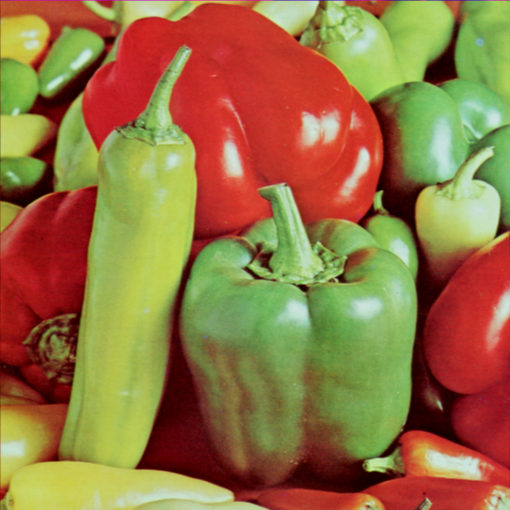
\includegraphics[width=\textwidth]{./imágenes/blurred.png}
    \end{subfigure}
    \hfill
    \begin{subfigure}{0.45\textwidth}
      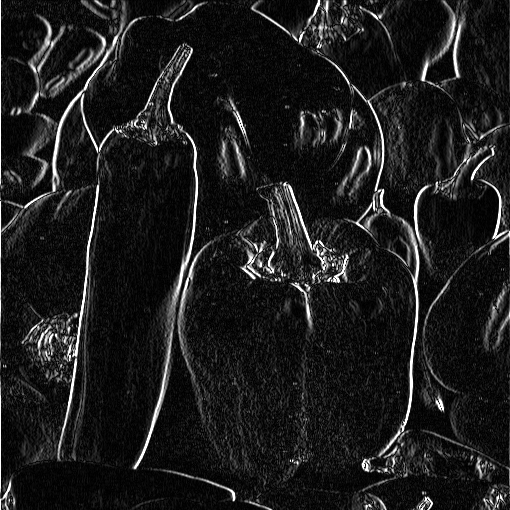
\includegraphics[width=\textwidth]{./imágenes/edged.png}
    \end{subfigure}
    \caption{Aplicación de filtros con sumador exacto.}
  \end{subfigure}
  % MAX DEPTH 3
  \begin{subfigure}{0.7\textwidth}
    \centering
    \begin{subfigure}{0.45\textwidth}
      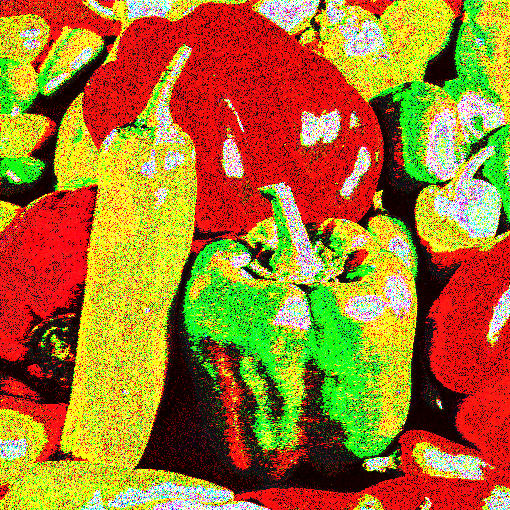
\includegraphics[width=\textwidth]{./imágenes/blurred_approx_3_one_tree_per_output.png}
      \caption*{SSIM=0.18}
    \end{subfigure}
    \hfill
    \begin{subfigure}{0.45\textwidth}
      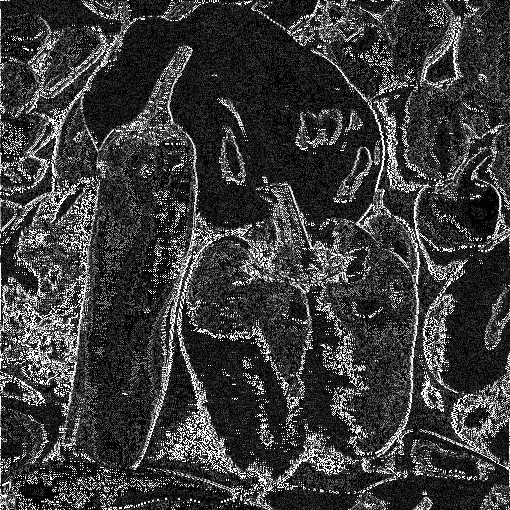
\includegraphics[width=\textwidth]{./imágenes/edged_approx_3_one_tree_per_output.png}
      \caption*{SSIM=0.17}
    \end{subfigure}
    \centering
    \caption{Profundidad máxima=3; Un árbol por salida=sí; MRED=27.3\%; MED=149.2; Área=59.73\%}
  \end{subfigure}

  % MAX DEPTH 4
  \begin{subfigure}{0.7\textwidth}
    \centering
    \begin{subfigure}{0.45\textwidth}
      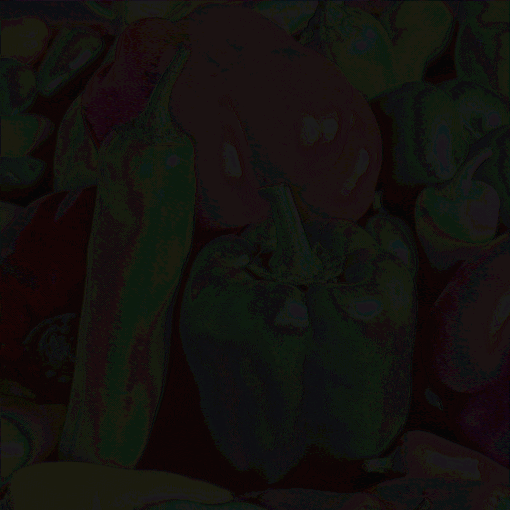
\includegraphics[width=\textwidth]{./imágenes/blurred_approx_4.png}
      \caption*{SSIM=0.05}
    \end{subfigure}
    \hfill
    \begin{subfigure}{0.45\textwidth}
      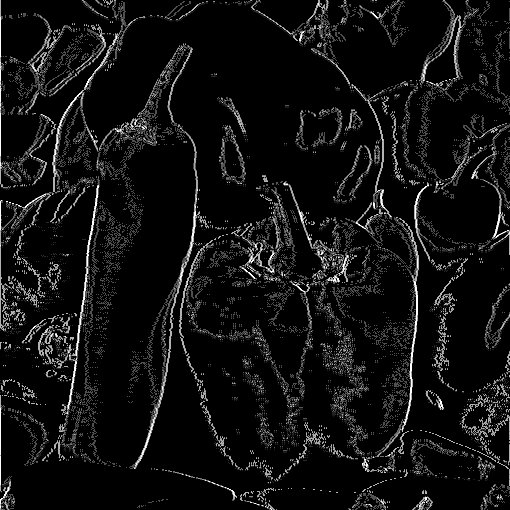
\includegraphics[width=\textwidth]{./imágenes/edged_approx_4.png}
      \caption*{SSIM=0.17}
    \end{subfigure}
    \centering
    \caption{Profundidad máxima=4; Un árbol por salida=no; MRED=24.2\%; MED=161.4; Área=49.61\%}
  \end{subfigure}

  \caption{Uso de sumadores aproximados con método de DT para la aplicación del filtro de desenfoque gaussiano (izquierda) y el filtro de detección de bordes Sobel (derecha).}
\label{fig:filters}
\end{figure}

Para demostrar una aplicación real del método de DT para la generación de
circuitos aproximados, en la Figura \ref{fig:filters} se presentan ejemplos de
su uso en aplicaciones de procesamiento de imágenes. Se muestran los resultados
de aplicar un filtro de desenfoque gaussiano y un filtro de detección de bordes
Sobel a una imagen, primero con un sumador exacto y luego con dos sumadores
aproximados distintos generados con DT. Los porcentajes de área mostrados en la
imagen son relativos al circuito BK\_16b, que era el sumador de 16 bits de menor
área entre los disponibles.

Para estos ejemplos, los DT se entrenaron con un conjunto de datos que contenía
todas las parejas de sumas posibles de 8 bits, y luego valores aleatorios
seleccionados entre 9 y 12 bits, ya que no era necesario sumar valores mayores.
Esto se debe a que los píxeles individuales tienen valores de 8 bits, pero las
sumas requeridas alcanzaban un valor máximo de \num{4080}, el cual requiere 12
bits para su representación.

El kernel utilizado para el filtro gaussiano se presenta en la siguiente matriz:

$$K = \begin{pmatrix} 1 & 2 & 1 \\ 2 & 4 & 2 \\ 1 & 2 & 1 \end{pmatrix}.$$

Este kernel fue escogido porque permite aplicar el filtro sin necesidad de un
multiplicador, ya que las multiplicaciones pueden realizarse únicamente con
corrimientos a la izquierda. Esto lo hace más representativo de una aplicación
real donde se utilice un sumador aproximado. Como un multiplicador es
considerablemente más complejo que un sumador, usar un sumador aproximado junto
con un multiplicador exacto resultaría en ganancias mínimas de área. Para el
filtro Sobel también se evitó el uso de multiplicaciones.

Como se puede observar, al utilizar un DT de profundidad 3 con un árbol
diferente por salida, se obtiene un resultado visualmente muy distinto al
obtenido con un DT de profundidad 4 que usa un solo árbol multi-salida. Esto
ocurre a pesar de que ambos circuitos aproximados tienen métricas similares de
MRED y MED.

También se incluyó en la figura la métrica SSIM (Índice de similitud
estructural) como una medida objetiva de la similitud entre los resultados
obtenidos con un sumador aproximado y el resultado exacto. Se aprecia que,
aunque el circuito generado por el DT con profundidad máxima 4 tiene un valor
de MRED bajo, el resultado del filtro de desenfoque gaussiano presenta un valor
de SSIM mucho menor que el obtenido con el DT de profundidad máxima 3, y
visualmente la imagen resultante apenas se puede distinguir. Esto constituye
otro ejemplo de cómo las métricas pueden ocultar detalles importantes. También
muestra que, aunque usar un árbol por salida suele generar peores métricas,
puede ser altamente beneficioso dependiendo de la aplicación.

En la Figura \ref{fig:comparacion_tiempos} se comparan
tiempos de ejecución para obtener los resultados mostrados en las tablas
anteriores. Se observa que el método \texttt{decision\_tree} es el que tuvo
ejecuciones más largas. Cabe notar que para \texttt{decision\_tree} se utilizó
un set de datos ajustado para que la simulación durase $\SI{20}{\second}$, en
vez de los $\SI{2}{\second}$ de simulación a los que se ajustaron los otros
métodos. Esto se hizo porque el método \texttt{decision\_tree} solo realiza 2
simulaciones por ejecución, a diferencia de los otros métodos que realizan una
por iteración y realizan múltiples iteraciones. De igual forma, la diferencia
en tiempos para circuitos más grandes supera los $\SI{40}{\second}$ que el
método \texttt{decision\_tree} tomaría en simular, sumado a esto que el método
\texttt{decision\_tree} fue el más lento en circuitos pequeños como RCA\_4b e
int2float, donde todos los métodos realizan una simulación con el set de
entradas exhaustivas que pueden tener los circuitos, se puede concluir que la
diferencia en tiempos de ejecución no se debe a los tiempos de simulación.

Dado esto, parece indicar que el método \texttt{decision\_tree} dura más tiempo
que los otros debido a los tiempos de sintetización. Durante las ejecuciones se
observó que sintetizar el circuito generado por el DT tomaba mucho tiempo. Se
teoriza que esto se da porque el DT genera circuitos donde a cada bit de salida
se le asigna una SOP compleja directamente, lo cual resulta en una descripción
de un circuito muy inusual y compleja que no tiene variables intermedias que
reutilice.

\begin{figure}
  \centering
  \begin{subfigure}{0.75\textwidth}
    \centering
    \includesvg[inkscapelatex=false, width=\textwidth]{./imágenes/0.01_threshold_time_comparison.svg}
    \caption{Tiempos de ejecución para resultados de Tabla \ref{tab:1_porciento}.}
    \label{fig:01_tiempo}
  \end{subfigure}
  \begin{subfigure}{0.75\textwidth}
    \centering
    \includesvg[inkscapelatex=false, width=\textwidth]{./imágenes/0.25_threshold_time_comparison.svg}
    \caption{Tiempos de ejecución para resultados de Tabla \ref{tab:25_porciento}.}
    \label{fig:25_tiempo}
  \end{subfigure}
  \begin{subfigure}{0.75\textwidth}
    \centering
    \includesvg[inkscapelatex=false, width=\textwidth]{./imágenes/0.5_threshold_time_comparison.svg}
    \caption{Tiempos de ejecución para resultados de Tabla \ref{tab:50_porciento}.}
    \label{fig:50_tiempo}
  \end{subfigure}
  \caption{Resultados de aplicación de resíntesis con método \texttt{decision\_tree}.}
  \label{fig:comparacion_tiempos}
\end{figure}

% Agregar algo de tiempos de ejecución. Posiblemente incluyendo lo de los
% circuitos no incluidos

% # DT

% - ✅ Comparación de DT con/sin resíntesis
% - ✅ Comparación de DT con/sin one_tree_per_output

% # DT vs otros métodos

% 🌀 = un poco pero podría más

% ✅ Hablar de capacidad de controlar error
% ✅ Tablas generales de error/área para diferentes umbrales:
%    ✅ 0.01
%    ✅ 0.25
%    ✅ 0.5
% ✅ Hablar de que no hay circuitos nuevos para los umbrales de 5% y 10%
% 🌀 Hablar de circuitos para los que no funcionó.
% 🌀 Hablar de (no) efectividad con circuitos grandes
% 🌀 Qué tipos de circuitos sobresale DT
% 🌀 Qué tipos de circuitos DT no sirve
% ✅ Hablar de valores de error de validación
